% updated in April 2002 by Antje Endemann
% Based on CVPR 07 and LNCS, with modifications by DAF, AZ and elle, 2008 and AA, 2010, and CC, 2011; TT, 2014; AAS, 2016

\documentclass[runningheads]{llncs}
\usepackage{graphicx}
\usepackage{amsmath,amssymb} % define this before the line numbering.
\usepackage{color}
\usepackage[width=122mm,left=12mm,paperwidth=146mm,height=193mm,top=12mm,paperheight=217mm]{geometry}
\begin{document}
% \renewcommand\thelinenumber{\color[rgb]{0.2,0.5,0.8}\normalfont\sffamily\scriptsize\arabic{linenumber}\color[rgb]{0,0,0}}
% \renewcommand\makeLineNumber {\hss\thelinenumber\ \hspace{6mm} \rlap{\hskip\textwidth\ \hspace{6.5mm}\thelinenumber}}
% \linenumbers
\pagestyle{headings}
\mainmatter

\title{Penguin colony detection with deep learning.} % Replace with your title

\titlerunning{Technical Report}

\authorrunning{Hieu Le}

\author{Hieu Le}

%Please write out author names in full in the paper, i.e. full given and family names. 
%If any authors have names that can be parsed into FirstName LastName in multiple ways, please include the correct parsing, in a comment to the volume editors:
%\index{Lastnames, Firstnames}
%(Do not uncomment it, because you may introduce extra index items if you do that...)

\institute{Computer Science Department,Stony Brook University\\
	\email{ \{hle\}@cs.stonybrook.edu}
}


\maketitle

%\begin{abstract}
%The abstract should summarize the contents of the paper. LNCS guidelines
%indicate it should be at least 70 and at most 150 words. It should be set in 9-point
%font size and should be inset 1.0~cm from the right and left margins.
%\dots
%\keywords{We would like to encourage you to list your keywords within
%the abstract section}
%\end{abstract}
\section{2nd-May-2018 | Exp: Performance of the model as the amount of training data grows.}

The experiments are conducted 3 times independently. For each trial, all data is randomly divided into 5 folds. The last chunk of data is kept untouched for testing. The first fold is used for training the first model. The first and second are used for training the second model. Likewise, the third model is trained on three chunk of data and the fourth model trained on four. Thus, from the first model to the fourth model, each is introduced with more training data. All other settings are the same for all models.


\def\subFigSzab{\linewidth}
\def\subFigx{0.20\linewidth}
\begin{figure}[h] 
\centering
\makebox[\subFigx]{(a) 25\%}
\makebox[\subFigx]{(b) 50\%}
\makebox[\subFigx]{(c) 75\%}
\makebox[\subFigx]{(d) 100\%}\\
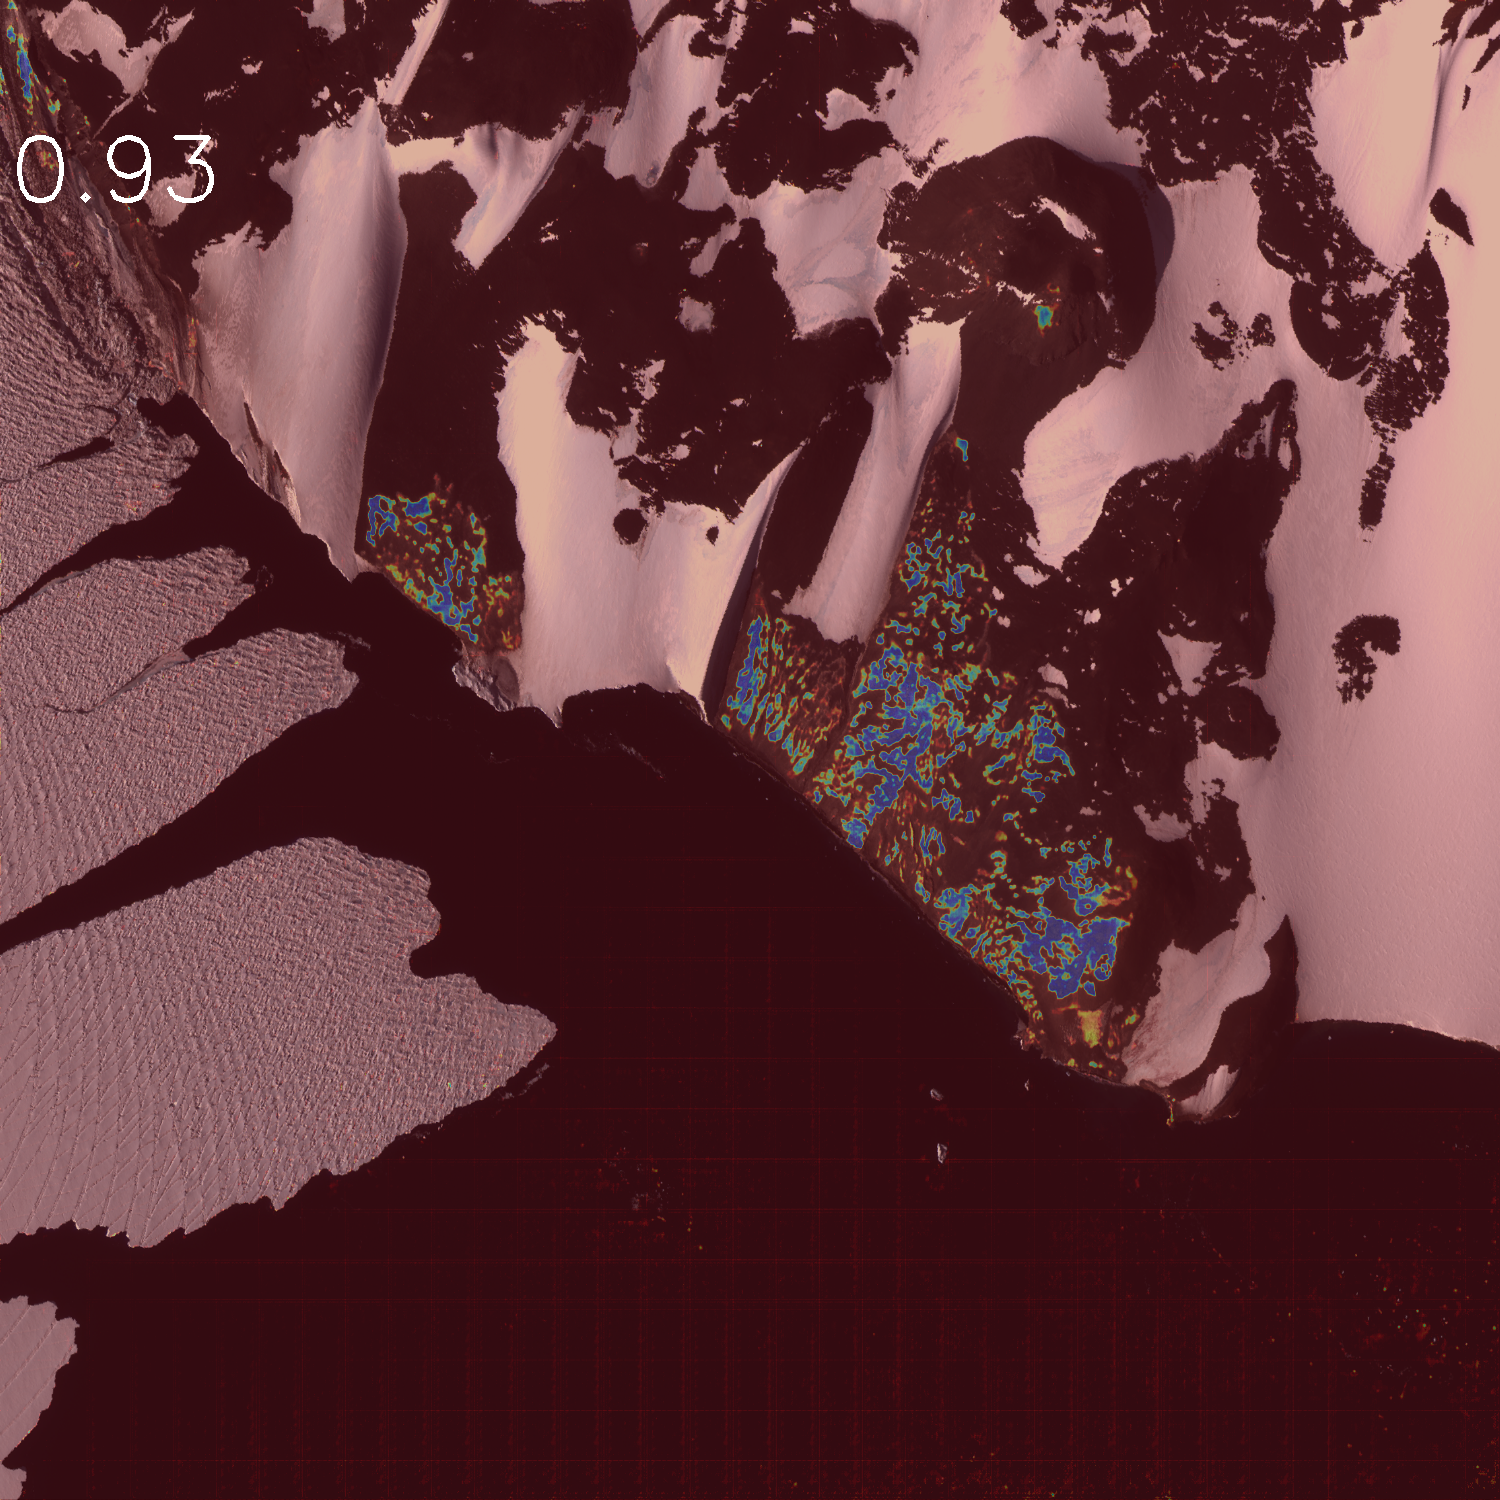
\includegraphics[width=\subFigx]{./fig/datagrow/MSE_single_unet_train_0_1.txt_bias-1_bs128_do0.1e25/WV02_20110131195115_1030010009CCF900_11JAN31195115-M1BS-052549143040_01_P003_u08rf3031.png}
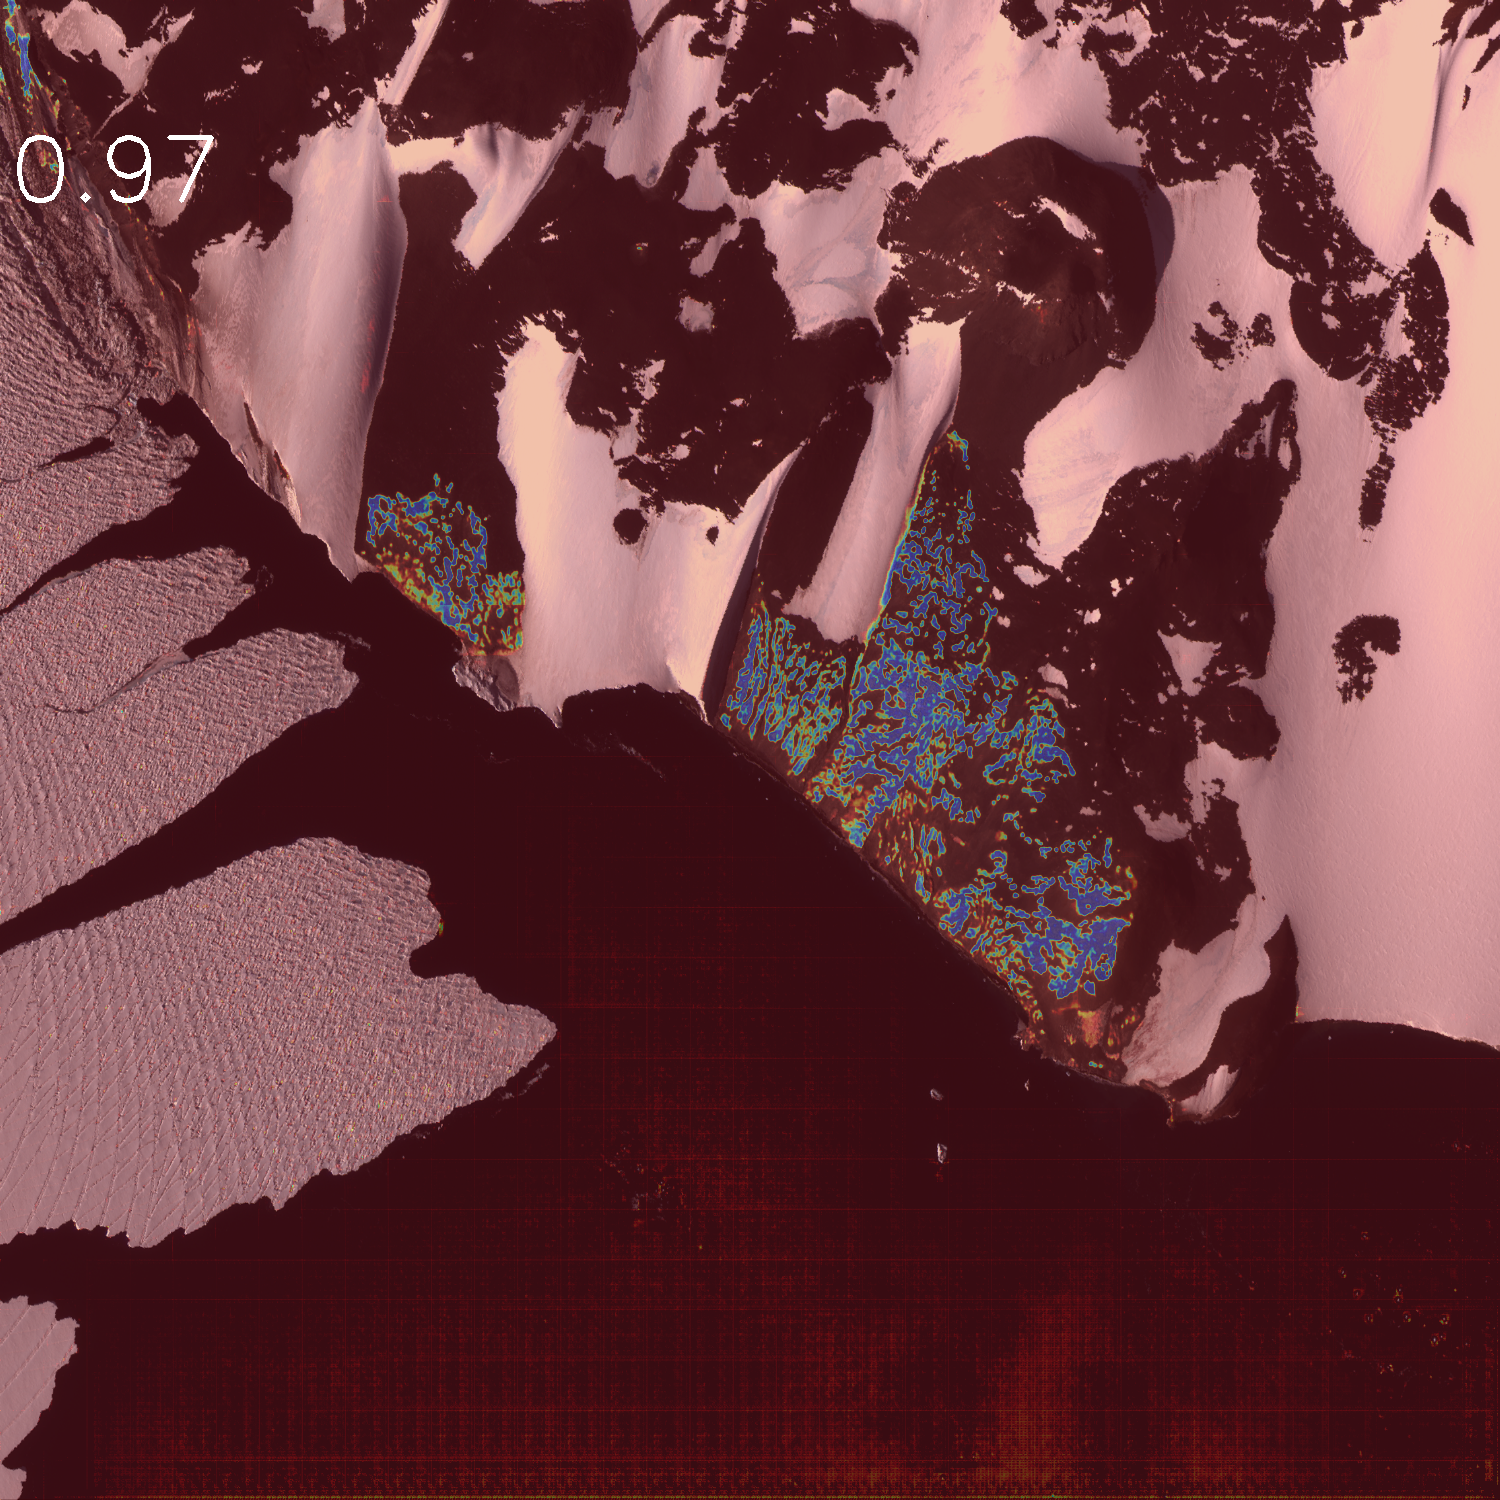
\includegraphics[width=\subFigx]{./fig/datagrow/MSE_single_unet_train_0_2.txt_bias-1_bs128_do0.1e25/WV02_20110131195115_1030010009CCF900_11JAN31195115-M1BS-052549143040_01_P003_u08rf3031.png}
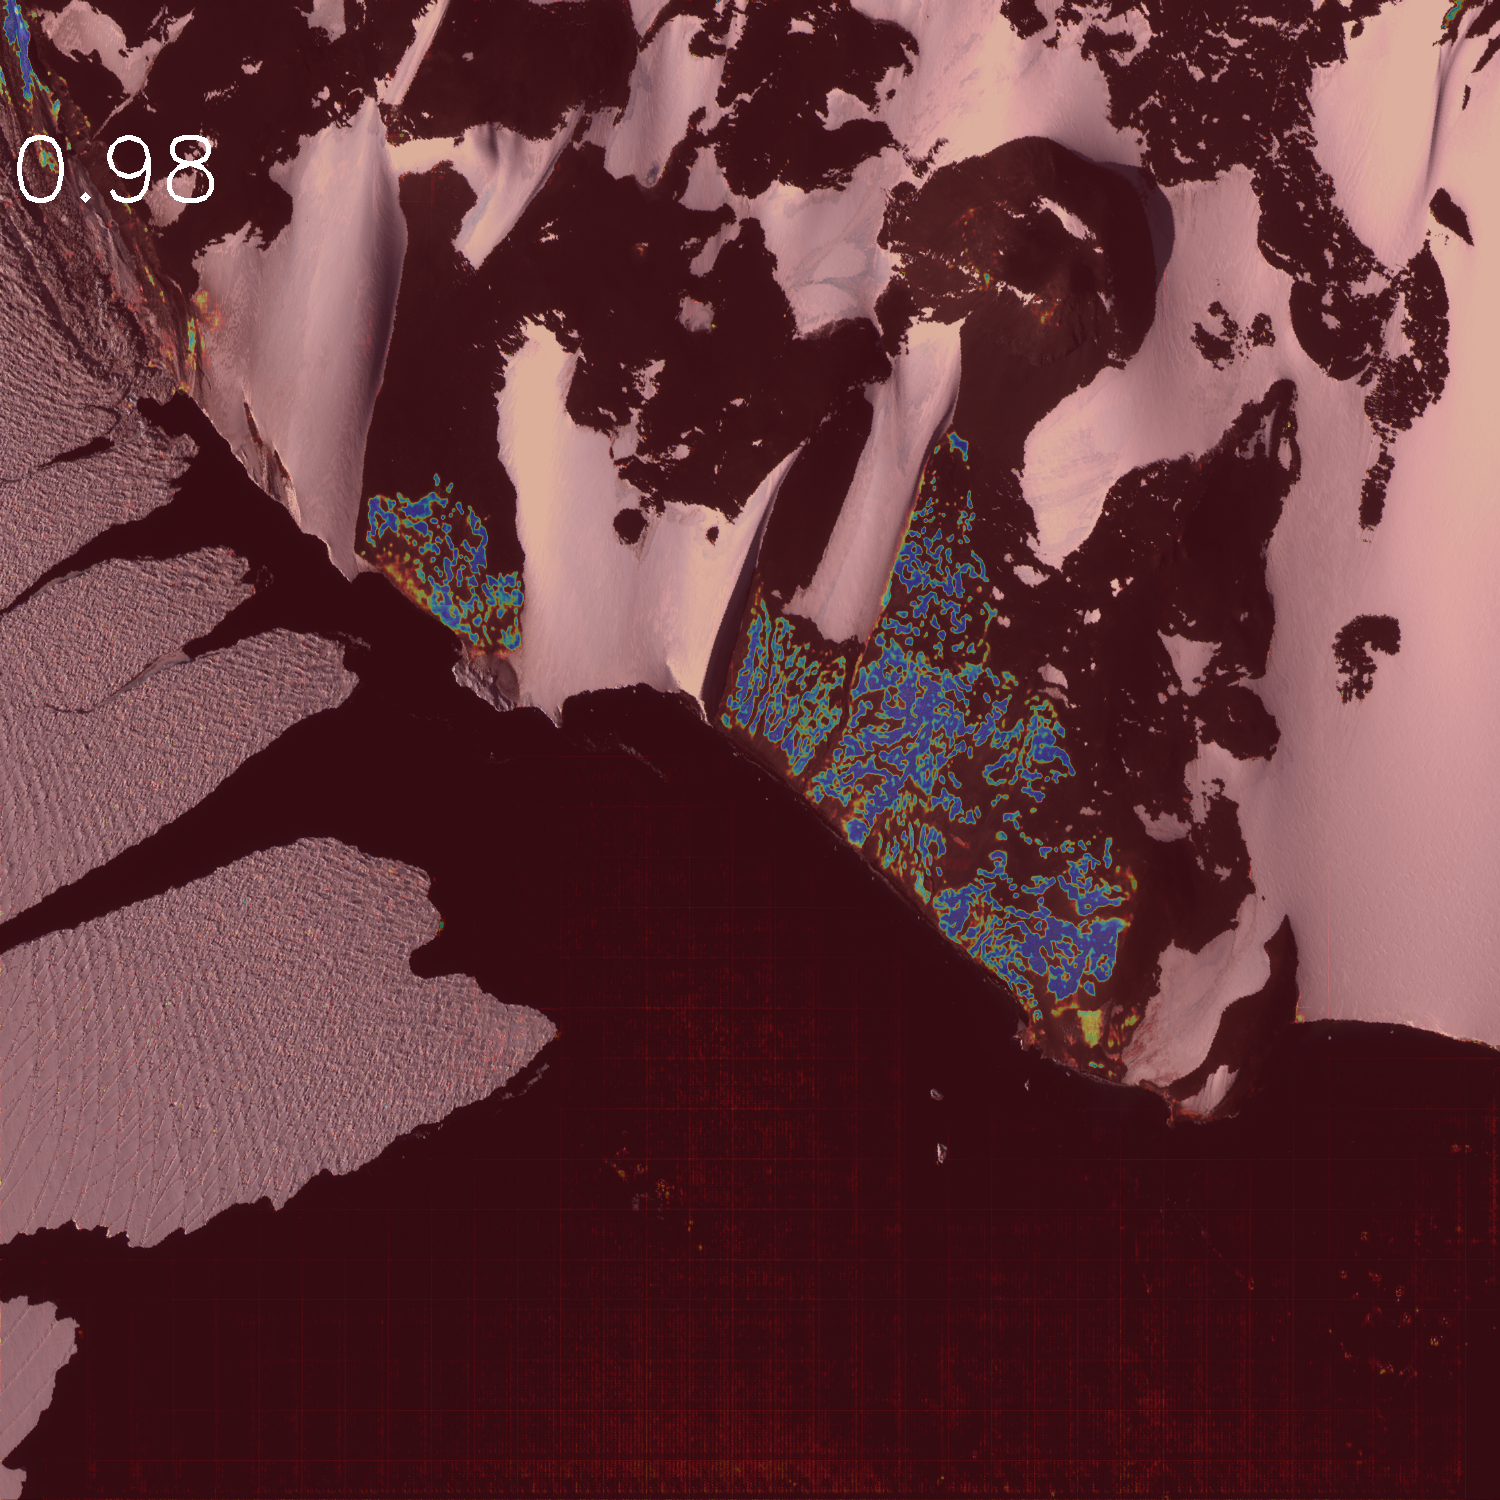
\includegraphics[width=\subFigx]{./fig/datagrow/MSE_single_unet_train_0_3.txt_bias-1_bs128_do0.1e25/WV02_20110131195115_1030010009CCF900_11JAN31195115-M1BS-052549143040_01_P003_u08rf3031.png}
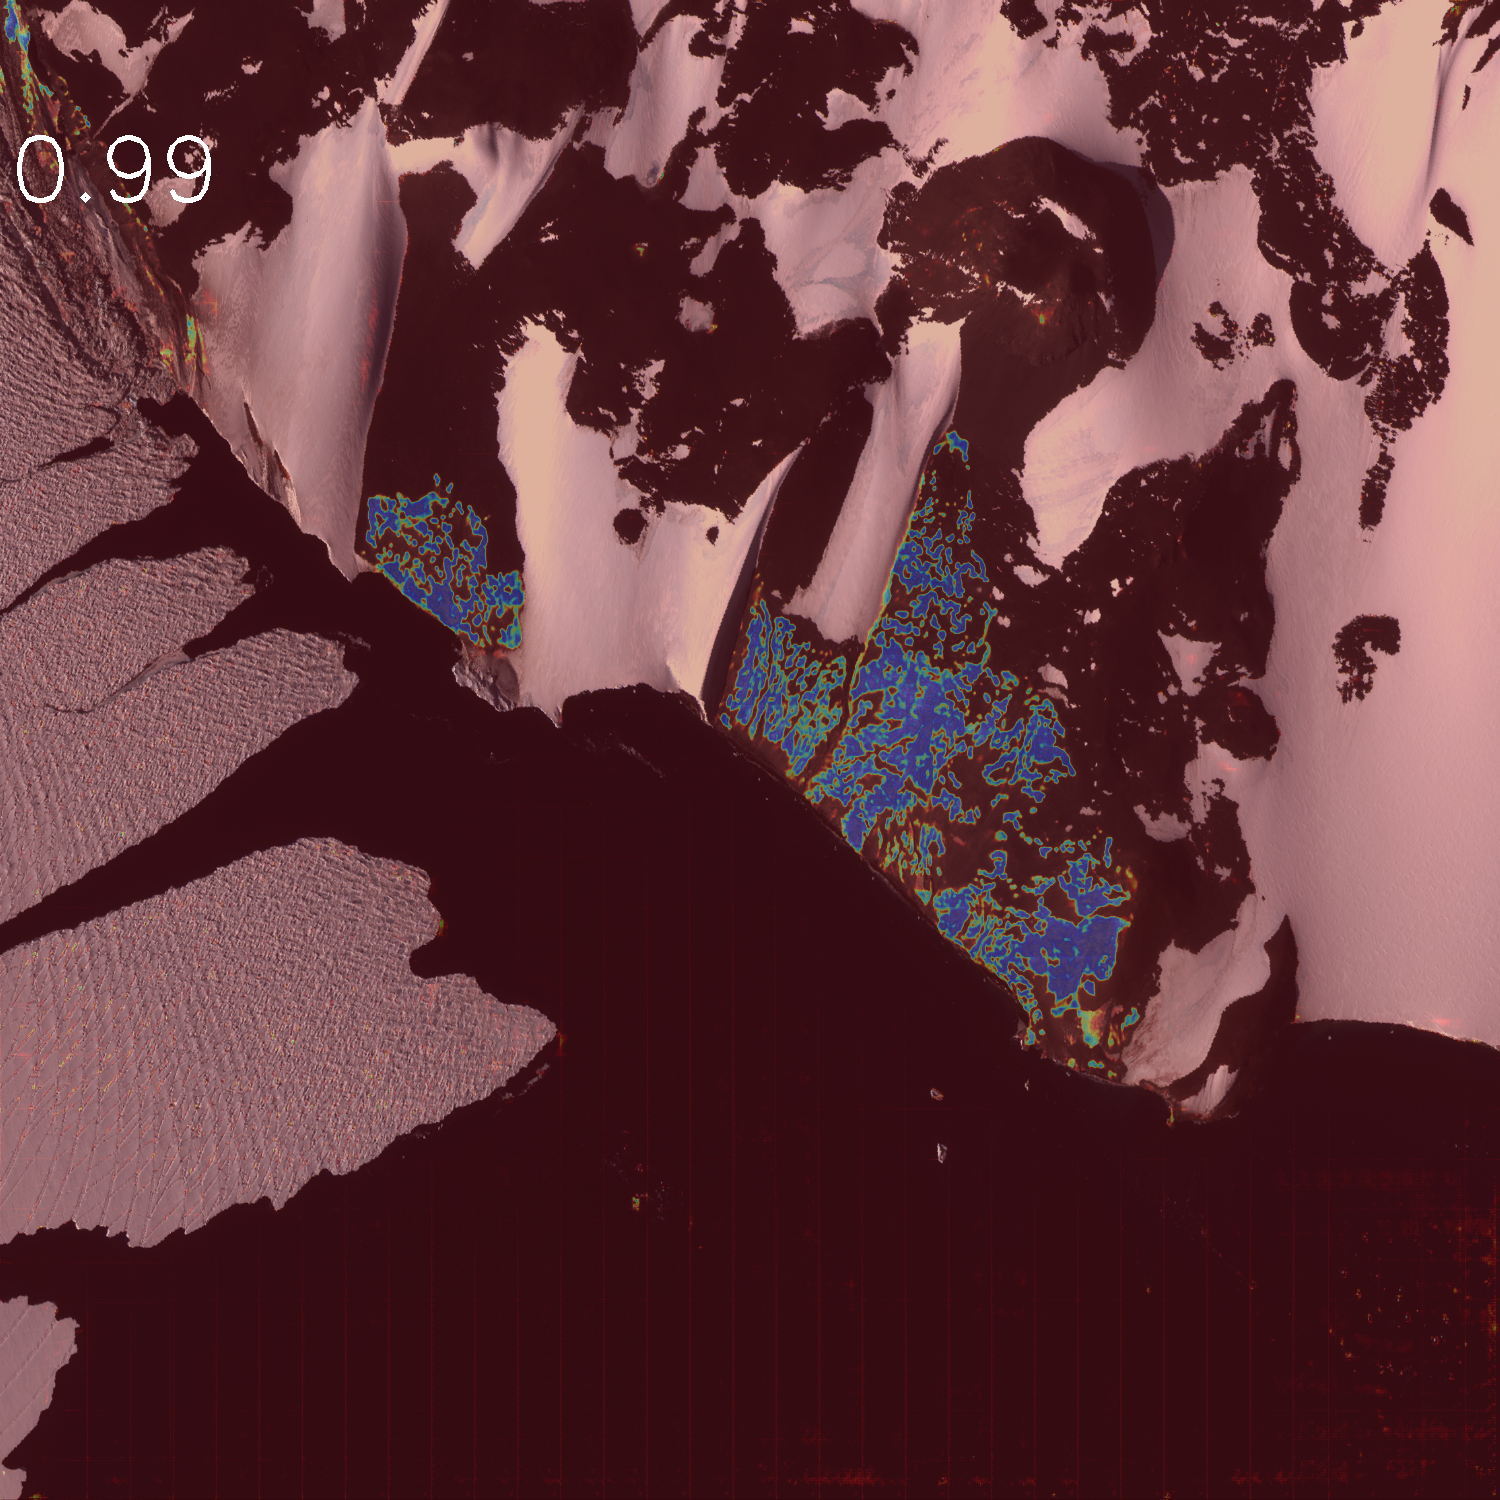
\includegraphics[width=\subFigx]{./fig/datagrow/MSE_single_unet_train_0_4.txt_bias-1_bs128_do0.1e25/WV02_20110131195115_1030010009CCF900_11JAN31195115-M1BS-052549143040_01_P003_u08rf3031.png}
\caption{{{\bf Performance of our model with different amount of training data.}}}
\label{fig:impress}
\end{figure}


\section{2nd-May-2018 | Exp: Varying dropout}

Dropout is a technique used in deep learning to reduce overfitting. For each training iteration, a percentage of units in each layer are selected to be deactivated as dropout means "dropping out units". This prevent complex co-adpataion on training data, or naively memorizing the training data, enforcing each unit to independently learn the features.

To understand the effect of dropout, we conduct two set of experiement with dropout = 0.5 and 0.2 respectively. 







\clearpage

\bibliographystyle{splncs03}
\bibliography{egbib}
\end{document}
